%%%%%%%%%%%%%%%%%%%%%%%%%%%%%%%%%%%%%%%%%%%%%%%%%%%%%%%%%%%%%%%%%%%%%%%%
%%                                                                    %%
%%                         ufersaTeX2                                 %%
%%                                                                    %%
%%              ATENÇÃO! Este modelo não é oficial!. 									%%
%%                                                                    %%
%% Este modelo não é um modelo oficial, trata-se de customizações do  %%
%% ueceTeX2 e abntTeX2 para adequar-se as normas da Universidade      %%
%% Federal Rural do Semi-árido (UFERSA). Feita de forma independente  %%
%% pelo aluno Josaias Moura (contato@josaiasmoura.com), aluno         %%
%% graduando em Engenharia de Software pela UFERSA, para auxiliar     %%
%% alunos da instituição em suas monografias. Ficando ele isento de   %%
%% quaisquer eventual responsabilidade por utilização deste modelo    %%
%% por terceiros.   																								  %%
%%                                                                    %%
%%              ATENÇÃO! Este modelo não é oficial!. 									%%
%%                                                                    %%
%% This work may be distributed and/or modified under the             %%
%% conditions of the LaTeX Project Public License, either version 1.3 %%
%% of this license or (at your option) any later version.             %%
%% The latest version of this license is in                           %%
%%   http://www.latex-project.org/lppl.txt                            %%
%% and version 1.3 or later is part of all distributions of LaTeX     %%
%% version 2005/12/01 or later.                                       %%
%%                                                                    %%
%% Agradecimentos aos responsáveis pelo ueceTeX2 e abntTeX2						%%
%%                                                                    %%
%%%%%%%%%%%%%%%%%%%%%%%%%%%%%%%%%%%%%%%%%%%%%%%%%%%%%%%%%%%%%%%%%%%%%%%%

%%%%%%%%%%%%%%%%%%%%%%%%%%%%%%%%%%%%%%%%%%%%%%%%%%%%%%%%%%%%%%%%%%%%%%%%
%%                                                                    %%
%%                         ufersaTeX2                                 %%
%%                                                                    %%
%%              ATENÇÃO! Este modelo não é oficial!. 									%%
%%                                                                    %%
%% Este modelo não é um modelo oficial, trata-se de customizações do  %%
%% ueceTeX2 e abntTeX2 para adequar-se as normas da Universidade      %%
%% Federal Rural do Semi-árido (UFERSA). Feita de forma independente  %%
%% pelo aluno Josaias Moura (contato@josaiasmoura.com), aluno         %%
%% graduando em Engenharia de Software pela UFERSA, para auxiliar     %%
%% alunos da instituição em suas monografias. Ficando ele isento de   %%
%% quaisquer eventual responsabilidade por utilização deste modelo    %%
%% por terceiros.   																								  %%
%%                                                                    %%
%%              ATENÇÃO! Este modelo não é oficial!. 									%%
%%                                                                    %%
%% This work may be distributed and/or modified under the             %%
%% conditions of the LaTeX Project Public License, either version 1.3 %%
%% of this license or (at your option) any later version.             %%
%% The latest version of this license is in                           %%
%%   http://www.latex-project.org/lppl.txt                            %%
%% and version 1.3 or later is part of all distributions of LaTeX     %%
%% version 2005/12/01 or later.                                       %%
%%                                                                    %%
%% Agradecimentos aos responsáveis pelo ueceTeX2 e abntTeX2						%%
%%                                                                    %%
%%%%%%%%%%%%%%%%%%%%%%%%%%%%%%%%%%%%%%%%%%%%%%%%%%%%%%%%%%%%%%%%%%%%%%%%

\documentclass[
    a4paper,          % Tamanho da folha A4
    12pt,             % Tamanho da fonte 12pt
    chapter=TITLE,    % Todos os capitulos devem ter caixa alta
    section=TITLE,    % Todas as secoes devem ter caixa alta
    oneside,          % Usada para impressao em apenas uma face do papel
    english,          % Hifenizacoes em ingles
    spanish,          % Hifenizacoes em espanhol
    brazil            % Ultimo idioma eh o idioma padrao do documento
]{abntex2}

% Importações de pacotes
\usepackage[utf8]{inputenc}                         % Acentuação direta
\usepackage[T1]{fontenc}                            % Codificação da fonte em 8 bits
\usepackage{graphicx}                               % Inserir figuras
\usepackage{amsfonts, amssymb, amsmath}             % Fonte e símbolos matemáticos
\usepackage{booktabs}                               % Comandos para tabelas
\usepackage{verbatim}                               % Texto é interpretado como escrito no documento
\usepackage{multirow, array}                        % Múltiplas linhas e colunas em tabelas
\usepackage{indentfirst}                            % Endenta o primeiro parágrafo de cada seção.
\usepackage{listings}                               % Utilizar codigo fonte no documento
\usepackage{xcolor}
\usepackage{microtype}                              % Para melhorias de justificação?
\usepackage[portuguese,ruled,lined]{algorithm2e}    % Escrever algoritmos
\usepackage{algorithmic}                            % Criar Algoritmos
%\usepackage{float}                                  % Utilizado para criação de floats
\usepackage{amsgen}
\usepackage{lipsum}                                 % Usar a simulação de texto Lorem Ipsum
%\usepackage{titlesec}                               % Permite alterar os títulos do documento
\usepackage{tocloft}                                % Permite alterar a formatação do Sumário
\usepackage{etoolbox}                               % Usado para alterar a fonte da Section no Sumário
\usepackage[nogroupskip,nonumberlist,acronym]{glossaries}                % Permite fazer o glossario
\usepackage{caption}                                % Altera o comportamento da tag caption
\usepackage[alf, abnt-emphasize=bf, bibjustif, recuo=0cm, abnt-etal-cite=3, abnt-etal-list=0,abnt-etal-text=it]{abntex2cite}  % Citações padrão ABNT
%\usepackage[bottom]{footmisc}                      % Mantém as notas de rodapé sempre na mesma posição
%\usepackage{times}                                 % Usa a fonte Times
\usepackage{mathptmx}                               % Usa a fonte Times New Roman
%\usepackage{lmodern}                               % Usa a fonte Latin Modern
%\usepackage{subfig}                                % Posicionamento de figuras
%\usepackage{scalefnt}                              % Permite redimensionar tamanho da fonte
\usepackage{color, colortbl}                       % Comandos de cores
%\usepackage{lscape}                                % Permite páginas em modo "paisagem"
%\usepackage{ae, aecompl}                           % Fontes de alta qualidade
%\usepackage{picinpar}                              % Dispor imagens em parágrafos
%\usepackage{latexsym}                              % Símbolos matemáticos
%\usepackage{upgreek}                               % Fonte letras gregas
\usepackage{appendix}                               % Gerar o apendice no final do documento
\usepackage{paracol}                                % Criar paragrafos sem identacao
\usepackage{lib/ufersatex2}		                    % Biblioteca com as normas da UFERSA para trabalhos academicos
\usepackage{pdfpages}                               % Incluir pdf no documento
\usepackage{amsmath}                                % Usar equacoes matematicas


% Define linguagem JavaScript
\definecolor{lightgray}{rgb}{.9,.9,.9}
\definecolor{darkgray}{rgb}{.4,.4,.4}
\definecolor{purple}{rgb}{0.65, 0.12, 0.82}
\definecolor{mygreen}{rgb}{0.0, 0.5, 0.0}
\lstdefinelanguage{JavaScript}{
  keywords={typeof, new, true, false, catch, function, return, null, catch, switch, var, if, in, while, do, else, case, break, let, const},
  keywordstyle=\color{blue}\bfseries,
  ndkeywords={class, export, boolean, throw, implements, import, this},
  ndkeywordstyle=\color{darkgray}\bfseries,
  identifierstyle=\color{black},
  sensitive=false,
  comment=[l]{//},
  morecomment=[s]{/*}{*/},
  commentstyle=\color{purple}\ttfamily,
  stringstyle=\color{mygreen}\ttfamily,
  morestring=[b]',
  morestring=[b]"
}
\lstset{
   language=JavaScript,
   backgroundcolor=\color{lightgray},
   frame=l,
   extendedchars=true,
   %basicstyle=\footnotesize\ttfamily,
   basicstyle={\small\ttfamily},
   showstringspaces=false,
   showspaces=false,
   numbers=left,
   numberstyle=\footnotesize,
   numbersep=9pt,
   stepnumber=1,
   firstnumber=1,
   numberfirstline=true,
   tabsize=2,
   breaklines=true,
   showtabs=false,
   captionpos=b
}

% Organiza e gera a lista de abreviaturas, simbolos e glossario
\makeglossaries

% Gera o Indice do documento
\makeindex


%%%%%%%%%%%%%%%%%%%%%%%%%%%%%%%%%%%%%%%%%%%%%%%%%%%%%
%%          Configuracoes do ufersaTeX2            %%
%%%%%%%%%%%%%%%%%%%%%%%%%%%%%%%%%%%%%%%%%%%%%%%%%%%%%

\graduacaoem{Tecnologia da Informação} % Curso
\habilitacao{bacharel} % Pode colocar também 'licenciada'

% Recomendadas
\trabalhoacademico{tccgraduacao}
\ehqualificacao{nao}
\removerbordasdohyperlink{sim}
%\cordohyperlink{nao}

%%%%%%%%%%%%%%%%%%%%%%%%%%%%%%%%%%%%%%%%%%%%%%%%%%%%%
%%          Informação sobre a IES                 %%
%%%%%%%%%%%%%%%%%%%%%%%%%%%%%%%%%%%%%%%%%%%%%%%%%%%%%

\ies{Universidade Federal Rural Do Semi-Árido}
\iessigla{UFERSA}
\campus{Pau dos Ferros}
\centro{Departamento de Engenharias e Tecnologia}

%%%%%%%%%%%%%%%%%%%%%%%%%%%%%%%%%%%%%%%%%%%%%%
%%  Informação relacionadas ao trabalho     %%
%%%%%%%%%%%%%%%%%%%%%%%%%%%%%%%%%%%%%%%%%%%%%%

\autor{Nome Completo do(a) Autor(a)}
\titulo{TÍTULO: SUBTÍTULO}
\data{2018}
\local{Pau dos Ferros -- RN}

%%%%%%%%%%%%%%%%%%%%%%%%%%%%%%%%%%%%%%%%%%%%%
%%     Informação sobre o Orientador       %%
%%%%%%%%%%%%%%%%%%%%%%%%%%%%%%%%%%%%%%%%%%%%%

\orientador{Prof. Dr. João de Tal}
\orientadories{UFERSA}
\orientadorcentro{Departamento De Engenharias e Tecnologia - Pau dos Ferros}
\orientadorfeminino{nao} % Coloque 'sim' se for do sexo feminino

%%%%%%%%%%%%%%%%%%%%%%%%%%%%%%%%%%%%%%%%%%%%%
%%      Informação sobre o Co-orientador   %%
%%%%%%%%%%%%%%%%%%%%%%%%%%%%%%%%%%%%%%%%%%%%%

% Deixe o nome do coorientador (caso não tenha um)

\coorientador{}
\coorientadories{UFERSA}
\coorientadorcentro{Departamento De Engenharias e Tecnologia - Pau dos Ferros}
\coorientadorfeminino{nao} % Coloque 'sim' se for do sexo feminino

%%%%%%%%%%%%%%%%%%%%%%%%%%%%%%%%%%%%%%%%%%%%%
%%      Informação sobre a banca           %%
%%%%%%%%%%%%%%%%%%%%%%%%%%%%%%%%%%%%%%%%%%%%%

% Atenção! O membro um é o presidente da banca, por padrão já vem definido como sendo seu orientador e recomendamos não alterar. No entanto, para definir o presidente da banca manualmente, descomente as linhas imediatamente abaixo.
%\membrodabancaum{Prof. Dr. Pedro de tal}
%\membrodabancaumies{UFERSA}
%\membrodabancaumcentro{Departamento De Engenharias e Tecnologia - Pau dos Ferros}

\membrodabancadois{Prof. Dr. Francisco de Tal}
\membrodabancadoisies{UFERSA}
\membrodabancadoiscentro{Departamento De Engenharias e Tecnologia - Pau dos Ferros}

\membrodabancatres{Prof. Dr. Beltrano de Tal}
\membrodabancatresies{UFERSA}
\membrodabancatrescentro{Departamento De Engenharias e Tecnologia - Pau dos Ferros}

%\membrodabancaquatro{Membro da Banca Quatro}
%\membrodabancaquatroies{Universidade do Membro da Banca Quatro - SIGLA}
%\membrodabancaquatrocentro{Centro de Ciências e Tecnologia - CCT}


%%%%%%%%%%%%%%%%%%%%%%%%%%%%%%%%%%%%%%%%%%%%%

\begin{document}

	% Se o seu trabalho é em ingles, descomente a linha a seguir
	%\selectlanguage{english}

	% --- Elementos pré-textuais
	% Dica! Você pode comentar os elementos que não deseja utilizar.

	% Elementos pré-textuais
	\imprimircapa
	\imprimirfolhaderosto{}
	\imprimirfichacatalografica{elementos-pre-textuais/ficha-catalografica}
	\imprimirerrata{elementos-pre-textuais/errata}
	%\imprimirfolhadeaprovacaopdf{elementos-pre-textuais/folha-aprovacao} % adicionar PDF da folha de aprovação assinada e escaneada
	\imprimirfolhadeaprovacao % comente essa linha quando adicionar o pdf da folha de aprovação
	\imprimirdedicatoria{elementos-pre-textuais/dedicatoria}
	\imprimiragradecimentos{elementos-pre-textuais/agradecimentos}
	\imprimirepigrafe{elementos-pre-textuais/epigrafe}
	\imprimirresumo{elementos-pre-textuais/resumo}
	\imprimirabstract{elementos-pre-textuais/abstract}
	\imprimirlistadeilustracoes
	\imprimirlistadetabelas
	\imprimirlistadequadros
	\imprimirlistadeabreviaturasesiglas
	\imprimirlistadesimbolos{elementos-pre-textuais/lista-de-simbolos}
	\imprimirsumario

	% --- Elementos textuais
	% Dica! Você pode comentar os elementos que não deseja utilizar.
	% Dica! Você pode adicionar mais elementos apenas adicionando uma nova linha
	%   \input{elementos-textuais/nome-do-meu-novo-elemento}

	\textual
	\chapter{Introdução}
\label{cap:introducao}

Diante da mudança de foco da sociedade -do agrícola para o industrial, deste para o informacional e agora para o conhecimento- e dos novos modelos administrativos - participativo, democrático e misto - as empresas passaram a perceber a importância dos documentos e da informação, preocupando-se com a sua gestão e buscando uma maior organização, guarda e destinação. Consequentemente, o tratamento da informação passou a constar do planejamento estratégico das organizações do conhecimento em busca do acompanhamento das mudanças da atual Sociedade do Conhecimento.

\section{Motivação}
\label{sec:motivacao}

Lorem ipsum dolor sit amet, consectetur adipiscing elit. Pellentesque in consectetur quam. Duis a mi a mauris tempus pretium non sit amet dui. Ut malesuada ex at purus rhoncus fermentum. Pellentesque auctor diam ut mauris vestibulum, aliquet feugiat odio scelerisque. Lorem ipsum dolor sit amet, consectetur adipiscing elit. Donec feugiat enim sed elit facilisis molestie. Suspendisse sed nisl at ligula porttitor mattis.

\section{Objetivos}
\label{sec:objetivos}

\subsection{Objetivo Geral}
\label{sec:objetivo-geral}

Lorem ipsum dolor sit amet, consectetur adipiscing elit. Pellentesque in consectetur quam. Duis a mi a mauris tempus pretium non sit amet dui. Ut malesuada ex at purus rhoncus fermentum. Pellentesque auctor diam ut mauris vestibulum, aliquet feugiat odio scelerisque. Lorem ipsum dolor sit amet, consectetur adipiscing elit. Donec feugiat enim sed elit facilisis molestie. Suspendisse sed nisl at ligula porttitor mattis.

\subsection{Objetivos Específicos}
\label{sec:objetivos-especificos}

Lorem ipsum dolor sit amet, consectetur adipiscing elit. Duis scelerisque, velit at facilisis hendrerit, dui eros lacinia metus, non maximus mi tortor ut lectus. Donec hendrerit leo ut consectetur tincidunt.

	\begin{alineas}
		\item Lorem ipsum dolor sit amet, consectetur adipiscing elit. Nunc dictum sed tortor nec viverra.
		\item Praesent vitae nulla varius, pulvinar quam at, dapibus nisi. Aenean in commodo tellus. Mauris molestie est sed justo malesuada, quis feugiat tellus venenatis.
		\item Praesent quis erat eleifend, lacinia turpis in, tristique tellus. Nunc dictum sed tortor nec viverra.
		\item Mauris facilisis odio eu ornare tempor. Nunc dictum sed tortor nec viverra.
		\item Curabitur convallis odio at eros consequat pretium.
	\end{alineas}

	\section{Estrutura do trabalho}
	\label{sec:estrutura-do-trabalho}

	O presente trabalho foi organizado lorem ipsum dolor sit amet, consectetur adipiscing elit. Duis scelerisque, velit at facilisis hendrerit, dui eros lacinia metus, non maximus mi tortor ut lectus. Donec hendrerit leo ut consectetur tincidunt.

	\chapter{Fundamentação Teórica}
\label{cap:fundamentacao-teorica}

Integer non \textit{lacinia magna}. Aenean tempor lorem tellus, non sodales nisl commodo ut. Proin mattis placerat risus sit amet laoreet. Praesent sapien arcu, maximus ac fringilla efficitur, vulputate faucibus sem. Donec aliquet velit eros, sit amet elementum dolor pharetra eget. Integer eget mattis libero

\section{Fundamentação Teórica A}
\label{sec:fundamentacao-teorica-a}

Integer non \textit{lacinia magna}. Aenean tempor lorem tellus, non sodales nisl commodo ut. Proin mattis placerat risus sit amet laoreet. Praesent sapien arcu, maximus ac fringilla efficitur, vulputate faucibus sem. Donec aliquet velit eros, sit amet elementum dolor pharetra eget. Integer eget mattis libero na \cite{johnsen2005peer}.

	\begin{figure}[h!]
		\centering
		\Caption{\label{fig:bittorrent-2} Arquivo sendo distribuído utilizando  BitTorrent}
		\UFERSAfig{}{
			\fbox{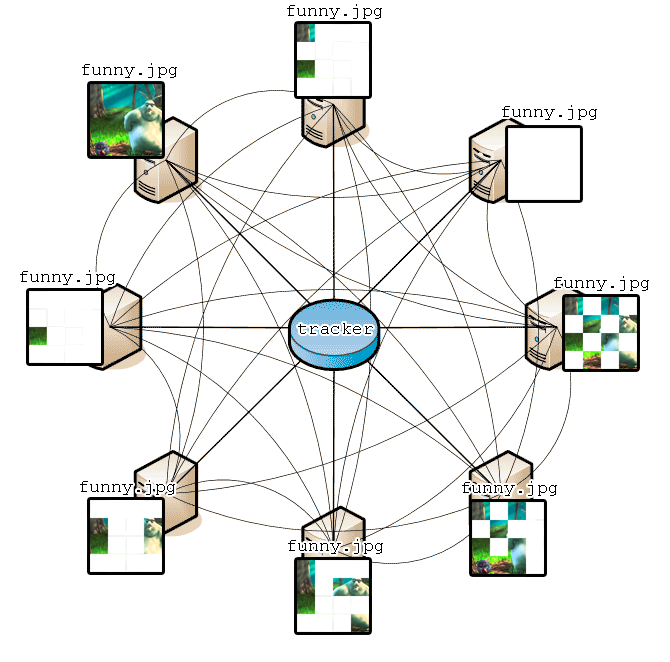
\includegraphics[width=10cm]{figuras/BITTORRENT_02}}
		}{
			\Fonte{Extraída de \citeonline{johnsen2005peer} e adaptada pelo autor}
		}
	\end{figure}

A Figura~\ref{fig:bittorrent-2}  mattis placerat risus sit amet laoreet. Praesent sapien arcu, maximus ac fringilla efficitur, vulputate faucibus sem. Donec aliquet velit eros, sit amet elementum dolor pharetra eget. Integer eget mattis libero na

\section{Fundamentação Teórica B}
\label{sec:fundamentacao-teorica-b}

Integer non lacinia magna. Aenean tempor lorem tellus, non sodales nisl commodo ut. Proin mattis placerat risus sit amet laoreet. Praesent sapien arcu, maximus ac fringilla efficitur, vulputate faucibus sem. Donec aliquet velit eros, sit amet elementum dolor pharetra eget. Integer eget mattis libero. Praesent ex velit, pulvinar at massa vel, fermentum dictum mauris. Ut feugiat accumsan

Nunc ac pretium dui. Mauris aliquam dapibus nulla ac mattis. Aenean non tortor volutpat, varius lectus vitae, accumsan nibh. Cras pretium vestibulum enim, id ullamcorper tortor ultrices non. Integer sodales viverra faucibus. Curabitur at dui lacinia, rhoncus lacus at, blandit metus. Integer scelerisque non enim quis ornare.

	\begin{table}[h!]
		\centering
		\Caption{\label{tab:end-privados} Intervalos de endereços privados reservados}
		\UFERSAtab{}{
			\begin{tabular}{lll}
				\toprule
				\multicolumn{2}{c}{Intervalo}&\\
				Limite inferior & Limite superior & Quantidade de hosts \\
				\midrule \midrule
				10.0.0.0	& 10.255.255.255	& 16.777.216 hosts\\
				172.16.0.0	& 172.31.255.255	& 1.048.576 hosts\\
				192.168.0.0	& 192.168.255.255	& 65.536 hosts\\
				\bottomrule
			\end{tabular}
		}{
			\Fonte{Adaptação extraída de \citeonline{rekhter1996address}}
		}
	\end{table}

Duis faucibus, enim quis tincidunt pellentesque, nisl leo varius nulla, vitae tempus dui mauris ac ante. Quisque purus lorem, pharetra sit amet lobortis eu, vehicula vitae purus.

Duis faucibus, enim quis tincidunt pellentesque, nisl leo varius nulla, vitae tempus dui mauris ac ante. Quisque purus lorem, pharetra sit amet lobortis eu, vehicula vitae purus: \acrlong{Bel}, \acrlong{Dr}, \acrlong{Esp}, \acrlong{GE}, \acrlong{GI}, \acrlong{IES}, \acrlong{Me}, \acrlong{SBGC}, \acrlong{UI}.

Duis faucibus, enim quis tincidunt pellentesque, nisl leo varius nulla, vitae tempus dui mauris ac ante. Quisque purus lorem, pharetra sit amet lobortis eu, vehicula vitae purus. Ut varius, erat nec vehicula elementum, risus est tempus justo, conforme ilustrado na Figura~\ref{fig:tanebaum-nat}.

\begin{figure}[h!]
	\centering
	\Caption{\label{fig:tanebaum-nat} Posicionamento e operação de um NAT}
	\UFERSAfig{}{
		\fbox{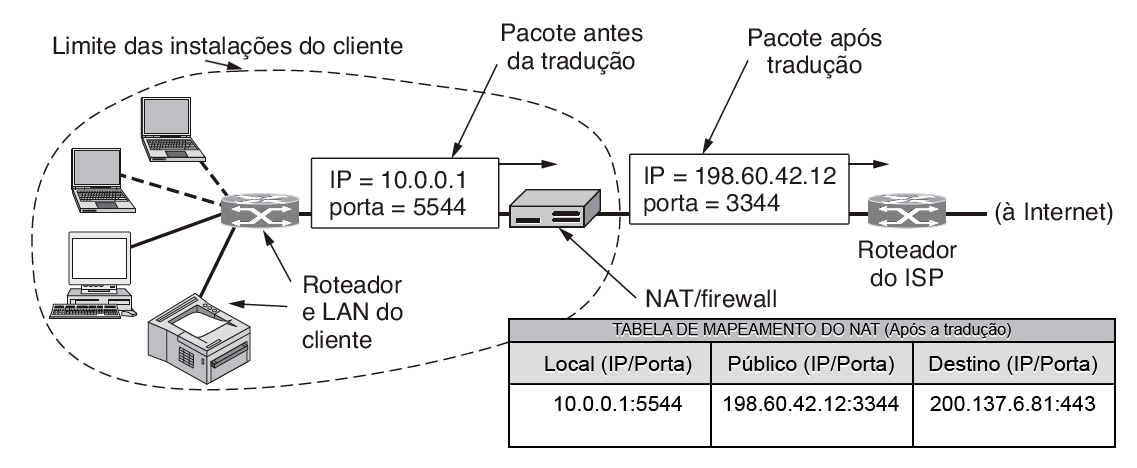
\includegraphics[width=13cm]{figuras/TANENBAUM_NAT_1}}
	}{
		\Fonte{Extraída de \citeonline{wetherall2011redes} alterado pelo autor}
	}
\end{figure}

	\chapter{Trabalhos Relacionados}
\label{cap:trabalhos-relacionados}

Lorem ipsum dolor sit amet, consectetur adipiscing elit. Pellentesque in consectetur quam. Duis a mi a mauris tempus pretium non sit amet dui. Ut malesuada ex at purus rhoncus fermentum. Pellentesque auctor diam ut mauris vestibulum, aliquet feugiat odio scelerisque. Lorem ipsum dolor sit amet, consectetur adipiscing elit. Donec feugiat enim sed elit facilisis molestie. Suspendisse sed nisl at ligula porttitor mattis.

\section{Trabalho Relacionado A}
\label{sec:trabalho-relacionado-a}

Lorem ipsum dolor sit amet, consectetur adipiscing elit. Pellentesque in consectetur quam. Duis a mi a mauris tempus pretium non sit amet dui. Ut malesuada ex at purus rhoncus fermentum. Pellentesque auctor diam ut mauris vestibulum, aliquet feugiat odio scelerisque. Lorem ipsum dolor sit amet, consectetur adipiscing elit. Donec feugiat enim sed elit facilisis molestie. Suspendisse sed nisl at ligula porttitor mattis.

\section{Trabalho Relacionado B}
\label{sec:trabalho-relacionado-b}

Lorem ipsum dolor sit amet, consectetur adipiscing elit. Pellentesque in consectetur quam. Duis a mi a mauris tempus pretium non sit amet dui. Ut malesuada ex at purus rhoncus fermentum. Pellentesque auctor diam ut mauris vestibulum, aliquet feugiat odio scelerisque. Lorem ipsum dolor sit amet, consectetur adipiscing elit. Donec feugiat enim sed elit facilisis molestie. Suspendisse sed nisl at ligula porttitor mattis.

	\begin{quadro}[h!]
		\centering
		\Caption{\label{qua:quadro-exemplo} Legenda do Quadro}
		\UFERSAqua{}{
			\begin{tabular}{|c|c|}
				\hline
				Nome & Texto \\
				\hline
				Maria & Duis a mi a mauris tempus pretium non sit amet dui  \\
				\hline
				João & Thoncus fermentum. Pellentesque auctor diam ut \\
				\hline
			\end{tabular}
		}{
			\Fonte{Elaborado pelo autor}
		}
	\end{quadro}

Lorem ipsum dolor sit amet, consectetur adipiscing elit. Pellentesque in consectetur quam. Duis a mi a mauris tempus pretium non sit amet dui. Ut malesuada ex at purus rhoncus fermentum. Pellentesque auctor diam ut mauris vestibulum, aliquet feugiat odio scelerisque. Lorem ipsum dolor sit amet, consectetur adipiscing elit. Donec feugiat enim sed elit facilisis molestie. Suspendisse sed nisl at ligula porttitor mattis. \gls{ambiguidade}, \gls{braile}.

	\chapter{Metodologia}
\label{chap:metodologia}

Lorem ipsum dolor sit amet, consectetur adipiscing elit. Pellentesque in consectetur quam. Duis a mi a mauris tempus pretium non sit amet dui. Ut malesuada ex at purus rhoncus fermentum. Pellentesque auctor diam ut mauris vestibulum, aliquet feugiat odio scelerisque. Lorem ipsum dolor sit amet, consectetur adipiscing elit. Donec feugiat enim sed elit facilisis molestie. Suspendisse sed nisl at ligula porttitor mattis.

O autor \cite{lamport1986latex} e \cite{Maia2011} Lorem ipsum dolor sit amet, consectetur adipiscing elit. Pellentesque in consectetur quam. Duis a mi a mauris tempus pretium non sit amet dui. Ut malesuada ex at purus rhoncus fermentum. Pellentesque auctor diam ut mauris vestibulum, aliquet feugiat odio scelerisque. Lorem ipsum dolor sit amet, consectetur adipiscing elit. Donec feugiat enim sed elit facilisis molestie. Suspendisse sed nisl at ligula porttitor mattis.

\cite{Huetal2000} lorem ipsum dolor sit amet, consectetur adipiscing elit. Pellentesque in consectetur quam. Duis a mi a mauris tempus pretium non sit amet dui. Ut malesuada ex at purus rhoncus fermentum. Pellentesque auctor diam ut mauris vestibulum, aliquet feugiat odio scelerisque. Lorem ipsum dolor sit amet, consectetur adipiscing elit. Donec feugiat enim sed elit facilisis molestie. Suspendisse sed nisl at ligula porttitor mattis.

\section{Exemplo de Algoritmos e Figuras}
\label{sec:exemplo-de-algoritmos-e-figuras}

Lorem ipsum dolor sit amet, consectetur adipiscing elit. Pellentesque in consectetur quam. Duis a mi a mauris tempus pretium non sit amet dui. Ut malesuada ex at purus rhoncus fermentum. Pellentesque auctor diam ut mauris vestibulum, aliquet feugiat odio scelerisque. Lorem ipsum dolor sit amet, consectetur adipiscing elit. Donec feugiat enim sed elit facilisis molestie. Suspendisse sed nisl at ligula porttitor mattis.

\begin{figure}[h!]
    \centering
    \Caption{\label{fig:codigo-exemplo} Exemplo de código JavaScript}
    \UFERSAfig{}{
        \fbox{\begin{minipage}{15cm}
        \lstinputlisting[language=JavaScript]{codigos/exemplo.js}
        \end{minipage}}
    }{
        \Fonte{O Autor, 2018}
    }
\end{figure}

Lorem ipsum dolor sit amet, consectetur adipiscing elit. Pellentesque in consectetur quam. Duis a mi a mauris tempus pretium non sit amet dui. Ut malesuada ex at purus rhoncus fermentum. Pellentesque auctor diam ut mauris vestibulum, aliquet feugiat odio scelerisque. Lorem ipsum dolor sit amet, consectetur adipiscing elit. Donec feugiat enim sed elit facilisis molestie. Suspendisse sed nisl at ligula porttitor mattis.

\section{Usando Fórmulas Matemáticas}

Lorem ipsum dolor sit amet, consectetur adipiscing elit. Pellentesque in consectetur quam. Duis a mi a mauris tempus pretium non sit amet dui. Ut malesuada ex at purus rhoncus fermentum. Pellentesque auctor diam ut mauris vestibulum, aliquet feugiat odio scelerisque. Lorem ipsum dolor sit amet, consectetur adipiscing elit. Donec feugiat enim sed elit facilisis molestie. Suspendisse sed nisl at ligula porttitor mattis.

	\begin{equation}
		\begin{aligned}
			x = a_0 + \cfrac{1}{a_1
				+ \cfrac{1}{a_2
					+ \cfrac{1}{a_3 + \cfrac{1}{a_4} } } }
		\end{aligned}
	\end{equation}

Lorem ipsum dolor sit amet, consectetur adipiscing elit. Pellentesque in consectetur quam. Duis a mi a mauris tempus pretium non sit amet dui. Ut malesuada ex at purus rhoncus fermentum. Pellentesque auctor diam ut mauris vestibulum, aliquet feugiat odio scelerisque. Lorem ipsum dolor sit amet, consectetur adipiscing elit. Donec feugiat enim sed elit facilisis molestie. Suspendisse sed nisl at ligula porttitor mattis.

	\begin{equation}
		\begin{aligned}
			k_{n+1} = n^2 + k_n^2 - k_{n-1}
		\end{aligned}
	\end{equation}

Lorem ipsum dolor sit amet, consectetur adipiscing elit. Pellentesque in consectetur quam. Duis a mi a mauris tempus pretium non sit amet dui. Ut malesuada ex at purus rhoncus fermentum. Pellentesque auctor diam ut mauris vestibulum, aliquet feugiat odio scelerisque. Lorem ipsum dolor sit amet, consectetur adipiscing elit. Donec feugiat enim sed elit facilisis molestie. Suspendisse sed nisl at ligula porttitor mattis.

	\begin{equation}
		\begin{aligned}
			\cos (2\theta) = \cos^2 \theta - \sin^2 \theta
		\end{aligned}
	\end{equation}

Lorem ipsum dolor sit amet, consectetur adipiscing elit. Pellentesque in consectetur quam. Duis a mi a mauris tempus pretium non sit amet dui. Ut malesuada ex at purus rhoncus fermentum. Pellentesque auctor diam ut mauris vestibulum, aliquet feugiat odio scelerisque. Lorem ipsum dolor sit amet, consectetur adipiscing elit. Donec feugiat enim sed elit facilisis molestie. Suspendisse sed nisl at ligula porttitor mattis.

	\begin{equation}
		\begin{aligned}
			A_{m,n} =
			\begin{pmatrix}
			a_{1,1} & a_{1,2} & \cdots & a_{1,n} \\
			a_{2,1} & a_{2,2} & \cdots & a_{2,n} \\
			\vdots  & \vdots  & \ddots & \vdots  \\
			a_{m,1} & a_{m,2} & \cdots & a_{m,n}
			\end{pmatrix}
		\end{aligned}
	\end{equation}

Lorem ipsum dolor sit amet, consectetur adipiscing elit. Pellentesque in consectetur quam. Duis a mi a mauris tempus pretium non sit amet dui. Ut malesuada ex at purus rhoncus fermentum. Pellentesque auctor diam ut mauris vestibulum, aliquet feugiat odio scelerisque. Lorem ipsum dolor sit amet, consectetur adipiscing elit. Donec feugiat enim sed elit facilisis molestie. Suspendisse sed nisl at ligula porttitor mattis.

	\begin{equation}
		\begin{aligned}
			f(n) = \left\{
			\begin{array}{l l}
			n/2 & \quad \text{if $n$ is even}\\
			-(n+1)/2 & \quad \text{if $n$ is odd}
			\end{array} \right.
		\end{aligned}
	\end{equation}

Lorem ipsum dolor sit amet, consectetur adipiscing elit. Pellentesque in consectetur quam. Duis a mi a mauris tempus pretium non sit amet dui. Ut malesuada ex at purus rhoncus fermentum. Pellentesque auctor diam ut mauris vestibulum, aliquet feugiat odio scelerisque. Lorem ipsum dolor sit amet, consectetur adipiscing elit. Donec feugiat enim sed elit facilisis molestie. Suspendisse sed nisl at ligula porttitor mattis.

\section{Usando Código-fonte}

Lorem ipsum dolor sit amet, consectetur adipiscing elit. Pellentesque in consectetur quam. Duis a mi a mauris tempus pretium non sit amet dui. Ut malesuada ex at purus rhoncus fermentum. Pellentesque auctor diam ut mauris vestibulum, aliquet feugiat odio scelerisque. Lorem ipsum dolor sit amet, consectetur adipiscing elit. Donec feugiat enim sed elit facilisis molestie. Suspendisse sed nisl at ligula porttitor mattis.

\begin{figure}[h!]
    \centering
    \Caption{\label{fig:codigo-exemplo} Exemplo de código Java}
    \UFERSAfig{}{
        \fbox{\begin{minipage}{15cm}
        \lstinputlisting[language=Java]{codigos/exemplo.java}
        \end{minipage}}
    }{
        \Fonte{O Autor, 2018}
    }
\end{figure}

Lorem ipsum dolor sit amet, consectetur adipiscing elit. Pellentesque in consectetur quam. Duis a mi a mauris tempus pretium non sit amet dui. Ut malesuada ex at purus rhoncus fermentum. Pellentesque auctor diam ut mauris vestibulum, aliquet feugiat odio scelerisque. Lorem ipsum dolor sit amet, consectetur adipiscing elit. Donec feugiat enim sed elit facilisis molestie. Suspendisse sed nisl at ligula porttitor mattis.

\section{Usando Teoremas, Proposições, etc}

Lorem ipsum dolor sit amet, consectetur adipiscing elit. Nunc dictum sed tortor nec viverra. consectetur adipiscing elit. Nunc dictum sed tortor nec viverra.

\begin{teo}[Pitágoras]
	Em todo triângulo retângulo o quadrado do comprimento da
	hipotenusa é igual a soma dos quadrados dos comprimentos dos catetos.
\end{teo}


Lorem ipsum dolor sit amet, consectetur adipiscing elit. Nunc dictum sed tortor nec viverra. consectetur adipiscing elit. Nunc dictum sed tortor nec viverra.

\begin{teo}[Fermat]
	Não existem inteiros $n > 2$, e $x, y, z$ tais que $x^n + y^n = z$
\end{teo}

Lorem ipsum dolor sit amet, consectetur adipiscing elit. Nunc dictum sed tortor nec viverra. consectetur adipiscing elit. Nunc dictum sed tortor nec viverra.

\begin{prop}
	Para demonstrar o Teorema de Pitágoras...
\end{prop}

Lorem ipsum dolor sit amet, consectetur adipiscing elit. Nunc dictum sed tortor nec viverra. consectetur adipiscing elit. Nunc dictum sed tortor nec viverra.

\begin{exem}
	Este é um exemplo do uso do ambiente exe definido acima.
\end{exem}

Lorem ipsum dolor sit amet, consectetur adipiscing elit. Nunc dictum sed tortor nec viverra. consectetur adipiscing elit. Nunc dictum sed tortor nec viverra.

\begin{xdefinicao}
	Definimos o produto de ...
\end{xdefinicao}

Lorem ipsum dolor sit amet, consectetur adipiscing elit. Nunc dictum sed tortor nec viverra. consectetur adipiscing elit. Nunc dictum sed tortor nec viverra.

\section{Usando Questões}

Lorem ipsum dolor sit amet, consectetur adipiscing elit. Nunc dictum sed tortor nec viverra. consectetur adipiscing elit. Nunc dictum sed tortor nec viverra.

\begin{questao}
	\item Esta é a primeira questão com alguns itens:
		\begin{enumerate}
			\item Este é o primeiro item
			\item Segundo item
		\end{enumerate}
	\item Esta é a segunda questão:
		\begin{enumerate}
			\item Este é o primeiro item
			\item Segundo item
		\end{enumerate}
	\item Lorem ipsum dolor sit amet, consectetur adipiscing elit. Nunc dictum sed tortor nec viverra. consectetur adipiscing elit. Nunc dictum sed tortor nec viverra.
		\begin{enumerate}
			\item consectetur
			\item adipiscing
			\item Nunc
			\item dictum
		\end{enumerate}
\end{questao}

\section{Citações}

\subsection{Documentos com três autores}

Quando houver três autores na citação, apresentam se os três, separados por ponto e vírgula, caso estes estejam após o texto. Se os autores estiverem incluídos no texto, devem ser separados por vírgula e pela conjunção "e".

\citeautoronline{tresautores}

\cite{tresautores}

\subsection{Documentos com mais de três autores}
Havendo mais de três autores, indica-se o primeiro seguido da expressão \textit{et al.} (do latim \textit{et alli}, que significa e outros), do ano e da página.

\citeautoronline{quatroautores}

\cite{quatroautores}

\subsection{Documentos de vários autores}

Havendo    citações    indiretas de    diversos    documentos    de    vários    autores, mencionados  simultaneamente e  que  expressam  a  mesma  ideia,  separam-se  os  autores  por ponto e vírgula, em ordem alfabética.

\cite{tresautores, quatroautores}

\section{Notas de Rodap\'{e}}

Deve-se utilizar o sistema autor-data para as  citações no texto e o numérico para notas explicativas\footnote{Veja - se como exemplo desse tipo de abordagem o estudo de Netzer (1976)}. As notas de rodapé podem e devem ser alinhadas, a partir da segunda linha da mesma nota, abaixo da primeira letra da primeira palavra, de forma a destacar o expoente \footnote{Encontramos  esse  tipo  de  perspectiva  na  2ª  parte  do  verbete  referido  na  nota  anterior,  em  grande  parte  do estudo de Rahner (1962).} e sem espaço entre elas e com fonte menor (tamanho 10).

	\chapter{Resultados}
\label{chap:resultados}

Lorem ipsum dolor sit amet, consectetur adipiscing elit. Pellentesque in consectetur quam. Duis a mi a mauris tempus pretium non sit amet dui. Ut malesuada ex at purus rhoncus fermentum. Pellentesque auctor diam ut mauris vestibulum, aliquet feugiat odio scelerisque. Lorem ipsum dolor sit amet, consectetur adipiscing elit. Donec feugiat enim sed elit facilisis molestie. Suspendisse sed nisl at ligula porttitor mattis.

\section{Resultados do Experimento A}
\label{sec:resultados-do-experimento-a}

Lorem ipsum dolor sit amet, consectetur adipiscing elit. Pellentesque in consectetur quam. Duis a mi a mauris tempus pretium non sit amet dui. Ut malesuada ex at purus rhoncus fermentum. Pellentesque auctor diam ut mauris vestibulum, aliquet feugiat odio scelerisque. Lorem ipsum dolor sit amet, consectetur adipiscing elit. Donec feugiat enim sed elit facilisis molestie. Suspendisse sed nisl at ligula porttitor mattis.

\begin{table}[h!]
  \centering
  \Caption{\label{tab:vm-config} Máquinas virtuais utilizadas nos testes}
  \UFERSAtab{}{
    \begin{tabular}{llll}
      \toprule
      Nome & Sistema Operacional & Memória alocada & Cores alocados \\
      \midrule \midrule
      Mininet-VM	        & Ubuntu (64-bit)	& 1024MB & 1 core\\
      NetworkEmulatorCore	& Ubuntu (32-bit)	& 2048MB & 2 cores \\
      \bottomrule
    \end{tabular}
  }{
    \Fonte{O Autor, 2018}
  }
\end{table}

\section{Resultados do Experimento B}
\label{sec:resultados-do-experimento-b}

Lorem ipsum dolor sit amet, consectetur adipiscing elit. Pellentesque in consectetur quam. Duis a mi a mauris tempus pretium non sit amet dui. Ut malesuada ex at purus rhoncus fermentum. Pellentesque auctor diam ut mauris vestibulum, aliquet feugiat odio scelerisque. Lorem ipsum dolor sit amet, consectetur adipiscing elit. Donec feugiat enim sed elit facilisis molestie. Suspendisse sed nisl at ligula porttitor mattis.

	\chapter{Conclusões e Trabalhos Futuros}
\label{chap:conclusoes-e-trabalhos-futuros}

Lorem ipsum dolor sit amet, consectetur adipiscing elit. Pellentesque in consectetur quam. Duis a mi a mauris tempus pretium non sit amet dui. Ut malesuada ex at purus rhoncus fermentum. Pellentesque auctor diam ut mauris vestibulum, aliquet feugiat odio scelerisque. Lorem ipsum dolor sit amet, consectetur adipiscing elit. Donec feugiat enim sed elit facilisis molestie. Suspendisse sed nisl at ligula porttitor mattis.

\section{Contribuições do Trabalho}
\label{sec:contribuicoes-do-trabalho}

Lorem ipsum dolor sit amet, consectetur adipiscing elit. Pellentesque in consectetur quam. Duis a mi a mauris tempus pretium non sit amet dui. Ut malesuada ex at purus rhoncus fermentum. Pellentesque auctor diam ut mauris vestibulum, aliquet feugiat odio scelerisque. Lorem ipsum dolor sit amet, consectetur adipiscing elit. Donec feugiat enim sed elit facilisis molestie. Suspendisse sed nisl at ligula porttitor mattis.

\section{Limitações}
\label{sec:limitacoes}

Lorem ipsum dolor sit amet, consectetur adipiscing elit. Pellentesque in consectetur quam. Duis a mi a mauris tempus pretium non sit amet dui. Ut malesuada ex at purus rhoncus fermentum. Pellentesque auctor diam ut mauris vestibulum, aliquet feugiat odio scelerisque. Lorem ipsum dolor sit amet, consectetur adipiscing elit. Donec feugiat enim sed elit facilisis molestie. Suspendisse sed nisl at ligula porttitor mattis.

\section{Trabalhos Futuros}
\label{sec:trabalhos-futuros}

Lorem ipsum dolor sit amet, consectetur adipiscing elit. Pellentesque in consectetur quam. Duis a mi a mauris tempus pretium non sit amet dui. Ut malesuada ex at purus rhoncus fermentum. Pellentesque auctor diam ut mauris vestibulum, aliquet feugiat odio scelerisque. Lorem ipsum dolor sit amet, consectetur adipiscing elit. Donec feugiat enim sed elit facilisis molestie. Suspendisse sed nisl at ligula porttitor mattis.


	% --- Elementos pós-textuais
	% Dica! Você pode comentar os elementos que não deseja utilizar.

	%Elementos pós-textuais
	\bibliography{elementos-pos-textuais/referencias}
	\imprimirglossario
	\imprimirapendices
		% Adicione aqui os apendices do seu trabalho
		\apendice{Histórico de mudanças}
\label{ap:historico}

Lorem ipsum dolor sit amet, consectetur adipiscing elit. Pellentesque in consectetur quam. Duis a mi a mauris tempus pretium non sit amet dui. Ut malesuada ex at purus rhoncus fermentum. Pellentesque auctor diam ut mauris vestibulum, aliquet feugiat odio scelerisque. Lorem ipsum dolor sit amet, consectetur adipiscing elit. Donec feugiat enim sed elit facilisis molestie. Suspendisse sed nisl at ligula porttitor mattis.

		\apendice{Lorem}
\label{ap:lorem-ipsum}

Lorem ipsum dolor sit amet, consectetur adipiscing elit. Pellentesque in consectetur quam. Duis a mi a mauris tempus pretium non sit amet dui. Ut malesuada ex at purus rhoncus fermentum. Pellentesque auctor diam ut mauris vestibulum, aliquet feugiat odio scelerisque. Lorem ipsum dolor sit amet, consectetur adipiscing elit. Donec feugiat enim sed elit facilisis molestie. Suspendisse sed nisl at ligula porttitor mattis.

	\imprimiranexos
		% Adicione aqui os anexos do seu trabalho
		\anexo{Exemplo de Anexo}
\label{an:exemplo-de-anexo}

Lorem ipsum dolor sit amet, consectetur adipiscing elit. Pellentesque in consectetur quam. Duis a mi a mauris tempus pretium non sit amet dui. Ut malesuada ex at purus rhoncus fermentum. Pellentesque auctor diam ut mauris vestibulum, aliquet feugiat odio scelerisque. Lorem ipsum dolor sit amet, consectetur adipiscing elit. Donec feugiat enim sed elit facilisis molestie. Suspendisse sed nisl at ligula porttitor mattis.

		\anexo{Exemplo de Anexo Dois}
\label{an:exemplo-de-anexo2}

Lorem ipsum dolor sit amet, consectetur adipiscing elit. Pellentesque in consectetur quam. Duis a mi a mauris tempus pretium non sit amet dui. Ut malesuada ex at purus rhoncus fermentum. Pellentesque auctor diam ut mauris vestibulum, aliquet feugiat odio scelerisque. Lorem ipsum dolor sit amet, consectetur adipiscing elit. Donec feugiat enim sed elit facilisis molestie. Suspendisse sed nisl at ligula porttitor mattis.

	\imprimirindice

\end{document}
